\documentclass[11pt]{article}
\usepackage{palatino, amsmath, setspace, graphicx, titling}
\usepackage[]{fullpage}
\usepackage{hyperref}
\usepackage[sort]{natbib} % for biblio

\newcommand{\subtitle}[1]{%
	\posttitle{%
		\par \end{center}
		\begin{center}\large#1\end{center}
		\vskip0.5em}%
	}


\begin{document}


\title{ Elastic deformation of a cylindrical hole in ice}
\subtitle{Based on Aadn\o{}y (1987), ``A complete elastic model for fluid-induced and in-situ generated stresses with the presence of a borehole.''  \textit{Energy Sources} vol. 9 pp. 239--259. }
\date{ \normalsize Begun November 10, 2016 at GSFC \\  Extensively updated during project visit, Buffalo, Oct. 31 -- Nov. 1, 2019 \\ Updated \today}
\author{\normalsize Kristin Poinar}

\maketitle


\onehalfspacing


\bigskip
Aadn\o{}y is interested in the stresses surrounding a borehole through porous, fluid-filled rock, for reasons of exploration safety.  He derives an analytic solution for the stress field near a cylindrical borehole through a solid (non-porous) medium, then goes on but we can stop there.  From the stress solution, it is straightforward to get the resulting strains using an elastic constitutive relation (Hooke's Law of Elasticity).

The  Aadn\o{}y paper is in our shared folders (Dropbox and Google and Github).

\section*{Aadn\o{}y's setup and stress solutions}

\begin{figure}
\begin{centering}
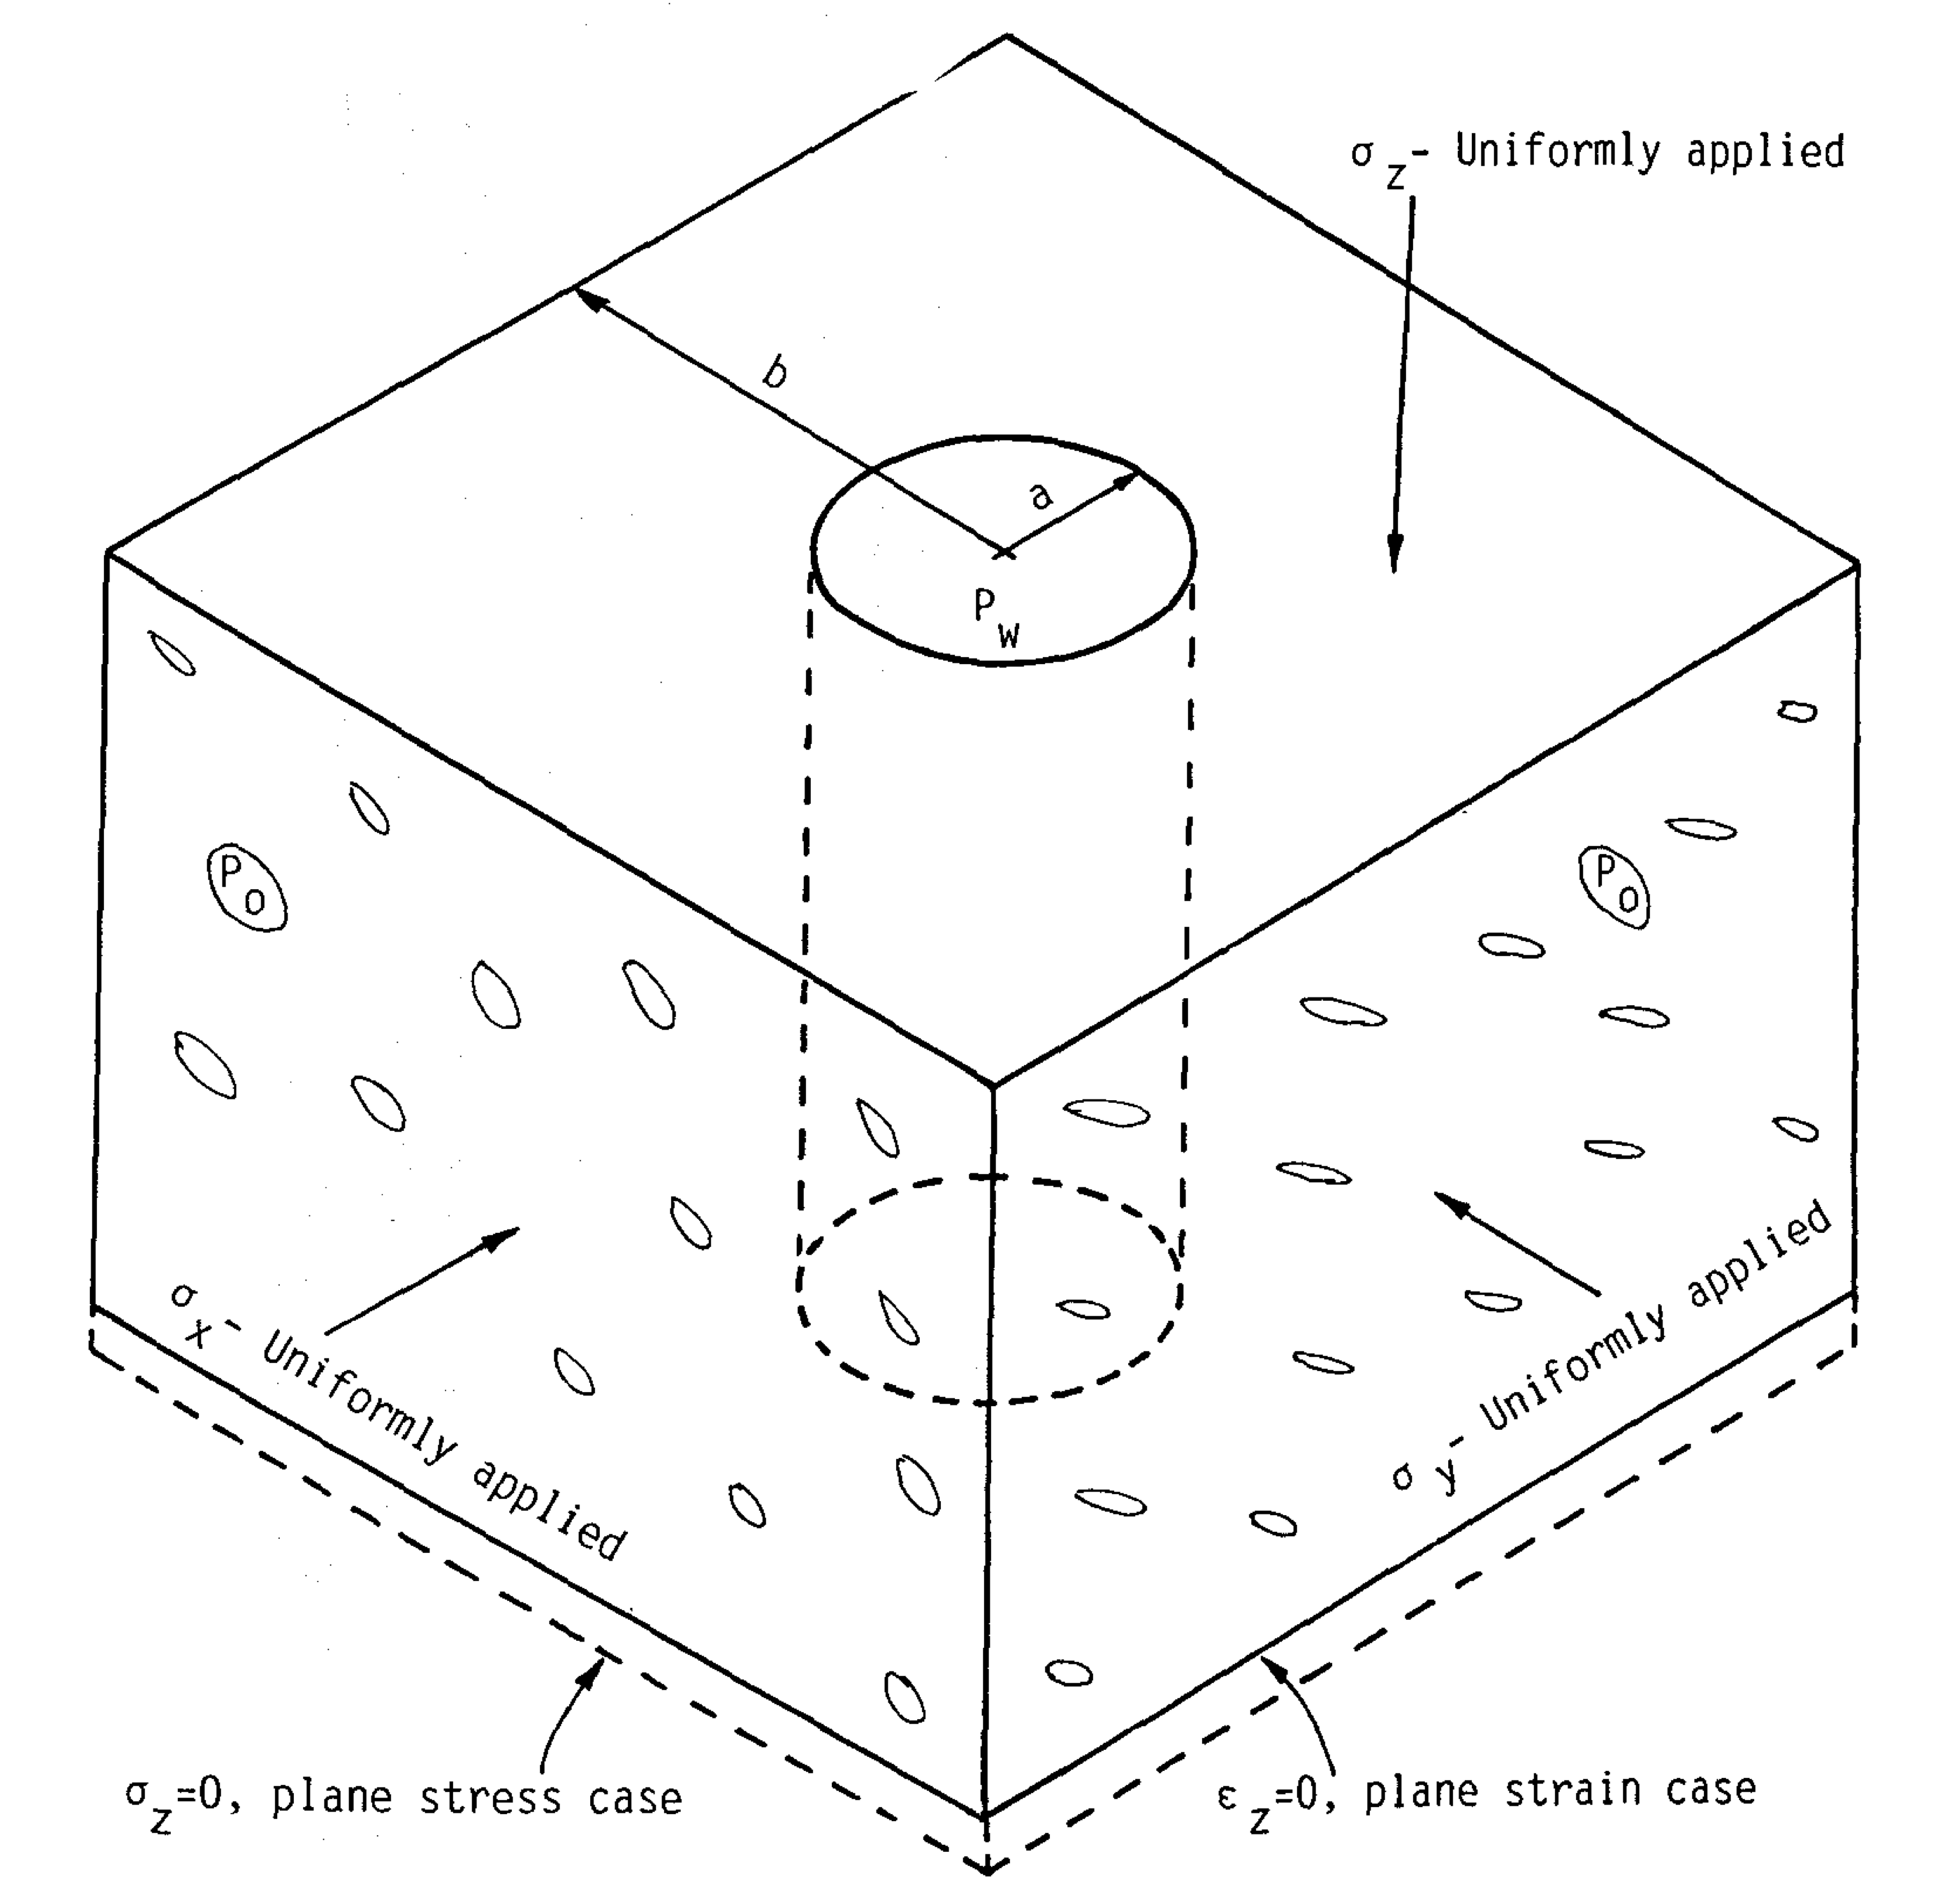
\includegraphics[width=0.55\textwidth]{AadnoyFigure1}
\caption{\textit{Setup, from Aadn\o{}y (1987).  His model is for a borehole in a porous rock medium, through which water can percolate.  That is why it has freckles.  We ignore pores.  We also use the plane strain case.}}
\end{centering}
\end{figure}

Aadn\o{}y finds the stress field around the borehole by summing the independent stress contributions from three sources: hydrostatic stress ($P$, which Aadn\o{}y thinks of as water pressure $P_w$; see end of document for expansion), deviatoric stresses ($\sigma_x$ and $\sigma_y$), and shear stress ($\tau_{xy}$).  The solution is in cylindrical coordinates ($r$, $\theta$, $z$).  Borehole radius is $a$.  

\begin{equation}
	\begin{aligned}
	\sigma_r &= \frac{\sigma_x+\sigma_y}{2}\left(1-\frac{a^2}{r^2}\right) + \frac{\sigma_x-\sigma_y}{2}\left(1+\frac{3a^4}{r^4}-\frac{4a^2}{r^2}\right) \cos2\theta + \tau_{xy}\left(1+\frac{3a^4}{r^4}-\frac{4a^2}{r^2}\right)\sin2\theta + \frac{a^2}{r^2}P \\
	\sigma_\theta &= \frac{\sigma_x+\sigma_y}{2}\left(1+\frac{a^2}{r^2}\right) - \frac{\sigma_x-\sigma_y}{2}\left(1+\frac{3a^4}{r^4}\right) \cos2\theta - \tau_{xy}\left(1+\frac{3a^4}{r^4}\right)\sin2\theta - \frac{a^2}{r^2}P \\
	\sigma_z &= \sigma_{zz} -2\nu\left(\sigma_x-\sigma_y\right)\frac{a^2}{r^2}\cos2\theta - 4\nu\tau_{xy}\frac{a^2}{r^2}\sin2\theta
	\end{aligned}
\label{StressSolutions}
\end{equation}

\noindent This assumes plane strain in $z$, i.e., the bottom of the ice has $\epsilon_z$=0 (no vertical deformation).  The stresses in $z$ are arranged such that this is possible (see the appearance of elastic parameter $\nu$ (Poisson's ratio) in the equation for $\sigma_z$).

These can be plugged into Hooke's Law to get the corresponding strain at any point in the domain.  Hooke's Law is just a linear combination of the three stresses in Eqn.~\ref{StressSolutions}:

\begin{equation}
	\begin{aligned}
	\epsilon_r &= E^{-1}\left(\sigma_r - \nu \left(\sigma_\theta + \sigma_z \right)\right) \\
	\epsilon_\theta &= E^{-1}\left(\sigma_\theta - \nu \left(\sigma_r + \sigma_z \right)\right) \\
	\epsilon_z &= E^{-1}\left(\sigma_z - \nu \left(\sigma_r + \sigma_\theta \right)\right)
	\end{aligned}
\label{Hooke}
\end{equation}

\noindent where $E$ is Young's modulus ($\sim$1~GPa) and $\nu$ is Poisson's ratio ($\sim$0.3, unitless).

\section*{Integrated elastic deformation}

We are interested in the total deformation of the borehole wall, or a spatially integrated version of $\epsilon_r$.  Deformation will be greatest at the borehole wall ($r=a$) and will fall off to zero as $r \rightarrow \infty$.  We would like to sum all these strains over the infinite distance of the ice block in order to get the total elastic deformation experienced from the borehole's perspective.  Integrating Eqn.~\ref{Hooke} over $r|_\infty^a$ entails integrating each stress from Eqn.~\ref{StressSolutions} over the same limits, then summing them together with some constants involved.  So, we would like to integrate all the \textit{r-dependent} terms in those stresses over these limits.  We can (and must) ignore any constant terms in Eqn.~\ref{StressSolutions} because these do not contribute to spatially varying deformation.  Also, integrating a constant over infinite limits makes an infinite result.

Eqn.~\ref{StressSolutions} with the constants removed are as follows:

\begin{equation}
	\begin{aligned}
	\sigma^*_r &= ~~~\left(P -  \frac{\sigma_x+\sigma_y}{2} \right)\left(\frac{a^2}{r^2}\right) + \left( \frac{\sigma_x-\sigma_y}{2}  \cos2\theta + \tau_{xy}\sin2\theta \right) \left(\frac{3a^4}{r^4}-\frac{4a^2}{r^2}\right)   \\
	\sigma^*_\theta &= - \left( P - \frac{\sigma_x+\sigma_y}{2}  \right) \left(\frac{a^2}{r^2}\right) - \left( \frac{\sigma_x-\sigma_y}{2} \cos2\theta + \tau_{xy}\sin2\theta \right) \left(\frac{3a^4}{r^4}\right)  \\
	\sigma^*_z &= \left( -2\nu\left(\sigma_x-\sigma_y\right)\cos2\theta - 4\nu\tau_{xy}\sin2\theta \right)  \left(\frac{a^2}{r^2} \right) 
	\end{aligned}
\label{StressStar}
\end{equation}

\noindent (It is just taking out all the $+1$s in the terms in parentheses.)

Indefinite integrals of Eqn.~\ref{StressStar} are easy, but I used Wolfram Alpha:

\begin{equation}
	\begin{aligned}
	\int \sigma^*_r dr &= \left( 2P - (\sigma_x+\sigma_y)  \right) \left( \frac{a^2}{2r} \right) + \left( (\sigma_x-\sigma_y) \cos2\theta + 2 \tau_{xy}\sin2\theta \right) \left( \frac{2a^2}{r} - \frac{3a^4}{2r^3} \right) \\
	\int \sigma^*_\theta dr &=  - \left( 2P - (\sigma_x+\sigma_y)  \right) \left( \frac{a^2}{2r} \right) + \left( (\sigma_x-\sigma_y) \cos2\theta + 2 \tau_{xy}\sin2\theta \right) \left(  \frac{3a^4}{2r^3} \right)  \\
	\int \sigma^*_z dr &= 2 \nu \left( \frac{a^2}{r} \right) \left( \left(\sigma_x-\sigma_y\right)\cos2\theta+2\tau_{xy}\sin2\theta\right)
	\end{aligned}
\label{IndefInt}
\end{equation}

\noindent These should all have dimensions of Pa$\cdot$m.

Definite integrals of Eqn.~\ref{IndefInt} go pretty smoothly, with everything in the $r\rightarrow\infty$ expressions going to zero.  Also, we don't care about tangential variations (coordinate $\theta$), so we will replace all $\cos2\theta$ or $\sin2\theta$ with its average absolute value, $\frac{1}{2}$.  We are left with

% Cos, Sin replaced with 1/2
\begin{equation}
	\begin{aligned}
	\int_\infty^r \sigma^*_r dr &=a \left(~~~P - \frac{1}{2} (\sigma_x + \sigma_y) + \frac{1}{4} (\sigma_x - \sigma_y)  + \frac{1}{2} \tau_{xy} \right) \\
	\int_\infty^r \sigma^*_\theta dr &= a \left(-P + \frac{1}{2} (\sigma_x + \sigma_y) + \frac{3}{4} (\sigma_x - \sigma_y)  + \frac{3}{4} \tau_{xy} \right) \\
	\int_\infty^r \sigma^*_z dr &= \nu a \left( \left(\sigma_x-\sigma_y\right) + 2 \tau_{xy}\right)
	\end{aligned}
\label{DefInt}
\end{equation}

So, finally we can take Eqn.~\ref{DefInt} and sum them all together with the appropriate elastic constants from Hooke's Law (Eqn.~\ref{Hooke}) to get the deformation in the $r$, $\theta$, and $z$ directions.  We only care about deformation in $r$, so that's all I'll do here.

\begin{equation}
	\begin{aligned}
	\int_\infty^a\epsilon_r dr &= E^{-1}\left[ \int_\infty^a \sigma^*_r dr - \nu\left( \int_\infty^a \sigma_\theta dr + \int_\infty^a \sigma_z dr \right)\right] \\
	u_r &=  \frac{a}{E} \left[ ( 1 + \nu ) \left( P - \frac{1}{2} (\sigma_x + \sigma_y) \right) + \frac{1}{4} (\sigma_x - \sigma_y) (1 - 3 \nu - 4 \nu^2) +   \frac{1}{4} \tau_{xy} (2 - 3 \nu - 8 \nu^2)\right]
	\end{aligned}
\label{DefVec}
\end{equation}

As a check, the integrated displacement, $u_r$ (Eq.~\ref{DefVec}), increases with moulin radius $a$.  This makes sense as the tighter the radius of curvature, the more difficult it is to deform.

Inward deformation (borehole closure) will have negative $u_r$ and outward deformation (growth of borehole) will have positive $u_r$.

With typical ice sheet values ($a\sim$1~meter; $\sigma_{x}$, $\sigma_y$ and $\tau_{xy}\sim$100~kPa; $P$ equivalent to $\sim$300--500~meters of water, with no cryostatic pressure), the total elastic deformation comes to a few millimeters, and it is outward (borehole opening).  In a borehole filled to flotation with $H_i-h_w$ = 30 meters of ice above the water line, elastic closure at the water line (where it is greatest) is half a millimeter.  %At the bottom of the borehole in that case

The elastic deformation happens essentially instantly.  In the model, it should happen inside a single timestep.  In the next timestep, a new moulin radius $a$ and a new water pressure will be provided based on the sums of all the other contributions, and we can recalculate the elastic displacement expected for that geometry.

I think it is just fine that $a$ will vary with depth (i.e., it is not a cylinder but a janky pipe of many diameters).

This solution, as written, does not include cryostatic pressure.   Aadn\o{}y calculated the stresses in an unweighted horizontal plate subjected to an environmental water pressure (think of a floppy disc at the bottom of a pool).  But I can easily modify $P$ to include the ice pressure as well as the water pressure.


\begin{equation}
	\begin{aligned}
	u_r &=  \frac{a}{E} \left[ ( 1 + \nu ) \left( P - \frac{1}{2} (\sigma_x + \sigma_y) \right) + \frac{1}{4} (\sigma_x - \sigma_y) (1 - 3 \nu - 4 \nu^2) +   \frac{1}{4} \tau_{xy} (2 - 3 \nu - 8 \nu^2)\right] \\
	P & = \rho_w g (h_w-z) - \rho_i g (H_i-z) = P_w - P_i
	\end{aligned}
\label{DeformationIceWaterPressures}
\end{equation}

\noindent The sign of the pressure $P$ is ``positive outward''.  That is, water pressure opens the borehole and ice pressure closes the borehole.





\section*{Next step: Creep deformation in a borehole using these stresses}

Resources are Ginny's exponential solution, which is currently implemented in the model using stresses similar to what you'd find at an ice shelf front, and the Fuenkajorn thesis from University of Arizona (\href{https://repository.arizona.edu/handle/10150/184451}{link}) titled ``Borehole closure in salt'', which is obviously more applicable to our cylindrical geometry.  

I also expect to be able to use the Aadn\o{}y stresses with Glen's Flow Law to get strain rates.  I don't know yet how to implement GFL in a cylindrical coordinate system, but I suppose it's relatively straightforward by applying a whole lot of coordinate system transformations (the standard ones I used to carry around with me in college) to the effective stresses, etc. for ice.  I'd expect these results to compare pretty well to the Arizona thesis.  (I believe salt has a nonlinear rheology, but I am not sure of its details.)










\end{document}